\documentclass[10pt]{iopart}

\usepackage{graphicx}
\graphicspath{{./figures/}}
%\usepackage[acronym]{glossaries}
\usepackage{acro}

\DeclareAcronym{cejst}{short=CEJST,
                       long=Climate and Energy Justice Screening Tool
}

\DeclareAcronym{ipcc}{short=IPCC,
                      long=International Panel on Climate Change
}

\DeclareAcronym{nsrdb}{short=NSRDB,
                       long=National Solar Radiation Database
}

\DeclareAcronym{nrel}{short=NREL,
                       long=National Renewable Energy Laboratory
}

\DeclareAcronym{lmi}{short=LMI,
                     long=low and moderate income
}

\DeclareAcronym{uhi}{short=UHI,
                     long=Urban Heat Island
}

\DeclareAcronym{ceja}{short=CEJA,
                      long=Climate and Equitable Jobs Act
}

\DeclareAcronym{ejscreen}{short=EJSCREEN,
                          long=Environmental Justice Screening Tool
}

\DeclareAcronym{epa}{short=EPA,
                     long=Environmental Protection Agency
}

% \usepackage[numbers]{natbib}
\usepackage{cite}
\usepackage{tabularx}
\usepackage{float}


\begin{document}

\title[Minimizing heatwave risk through an equitable distribution of solar panels]{Minimizing
heatwave risk through an equitable distribution of solar panels}

 \author{
 Samuel G. Dotson$^1$$^*$,
 Shannon R. Anderson$^2$,
 Alankrita Sahay$^3$,
 Pranjali Borse$^3$,
 Charumeghana Samantula$^3$
 }

 \address{ $^1$ Department of Nuclear, Plasma, and Radiological Engineering,
 University of Illinois Urbana-Champaign, Urbana IL, United States}
  \address{ $^2$ Department of  Natural Resources and Environmental Sciences,
 University of Illinois Urbana-Champaign, Urbana IL, United States}
  \address{ $^3$ Department of Civil and Environmental Engineering,
 University of Illinois Urbana-Champaign, Urbana IL, United States}
 \address{$^*$ Author to whom correspondence should be addressed}

 \ead{sgd2@illinois.edu}

 \begin{indented}
 \vspace{10pt}
 \item[]May 2022
 \end{indented}

 \begin{abstract}
Heat wave frequency and severity are increasing due to anthropogenic climate change.
Cities face higher consequences from heat waves because of the \ac{uhi} effect.
Rooftop solar panels are one method to mitigate \ac{uhi} and improve the adaptive
capacity of urban residents by lowering the cost of energy for low-income households.
This work uses a set of socioeconomic data, such as age, energy burden, population
density, and isolation, along with satellite temperature data, to identify regions
of high heat wave risk in Chicago so those regions may be prioritized for solar
panel subsidies from the state of Illinois. After curation, the data were clustered
using hierarchical clustering. The results of this process show improvements over
current prioritization schemes from the \ac{epa} \ac{ejscreen}. 
 \end{abstract}

 \vspace{2pc}
\noindent{\it Keywords}: solar, heatwave, equity, energy justice, policy

%\ioptwocol
\acresetall

\section{Introduction}
Climate change will increase the frequency and severity of extreme heat events and,
due to the \ac{uhi} effect, urban centers are more susceptible to heat waves and
heat stress \cite{zhao_strong_2014,dahl_killer_2019}. The Union of Concerned
Scientists estimates that the number of days above 32 $^\circ$C in the Midwest
will increase five-fold by midcentury unless action is taken to reduce carbon
emissions and slow climate change  \cite{dahl_killer_2019}. The lack of strong
federal climate policies leaves individual states and institutions responsible
for acting on climate change. This case study investigates the optimal distribution
of rooftop solar panels that minimizes heat wave risk for the City of Chicago.

We chose Chicago as the focus of this work for two reasons. First, Chicago was the
epicenter of a deadly heat wave in 1995; one of the deadliest heat waves in United
States history. Over 700 people died in this heat wave\cite{klinenberg_heat_2003}.
Further, the death toll from this heat wave was exacerbated by a combination of
social factors including income and isolation. As a result of this heat wave,
Chicago officials recognized the need to prepare for future heat waves. This
work proposes rooftop solar panels as a possible mitigation strategy.
Second, the State of Illinois has programs such as Solar for All and Illinois
Shines that aim to provide greater access to clean energy for low-income populations
\cite{illinois_solar_for_all_environmental_2022}. Thus, the resources to increase
rooftop solar penetration already exist but lack guidance based on heat wave risk.

Illinois Solar for All and Illinois Shines are two programs strengthened by the
2021 \ac{ceja} \cite{harmon_climate_2021}. These policies intend to expand the
rooftop solar capacity in Illinois by providing incentives or subsidies for solar
installation, with specific allocations for low-income communities. Rooftop solar
panels help reduce the percentage of household income spent on energy costs,
known as the energy burden, through net-metering policies that pay consumers for
excess energy generation \cite{brown_high_2020}. This reduction of energy burden
improves resilience to heat waves by increasing access to air-conditioning for
low-income households during high-demand times when electricity is most expensive.
However, a high penetration of intermittent renewables, such as solar panels,
increases price volatility and the energy burden for consumers without solar
installations. This is called the ``paradox of renewable energy policy'' and
highlights the need for efficient prioritization of at-risk areas \cite{blazquez_renewable_2018}.
Therefore, the purpose of this study is to identify areas with the highest heat
wave risk so they may be prioritized by programs like Solar for All and Illinois
Shines.

In order to identify high-priority areas, we curated economic and demographic
data for Chicago, along with satellite data from the \ac{nsrdb} published by the
\ac{nrel}. We perform hierarchical clustering on this data to identify regions of
similar risk and suitability for solar panels. Section \ref{section:methods_data}
discusses details of the data selection and processing, section \ref{section:results}
presents the results of the clustering algorithm, and section \ref{section:discussion}
develops a descriptive typology based on the clustered areas.


\section{Literature Review}
The \ac{uhi} effect, where urban areas tend to be warmer than their surroundings,
is one of the most evident impacts of human activity. Indeed, \ac{uhi} is one of
the most well studied phenomena, often using remote sensing technology and land
surface temperature data \cite{almeida_study_2021, cotlier_extreme_2022}.
Some studies evaluated \ac{uhi} intensity for particular cities by incorporating
data about urban features such as albedo, building height, and vegetation
\cite{sangiorgio_development_2020,abulibdeh_analysis_2021} along with urbanization
trends \cite{li_how_2021}. Other work in the literature examined \ac{uhi} along
a socio-economic axis.

\begin{itemize}
  \item What papers have looked at uhi and class?
  \item What papers have looked at uhi mitigation strategies?
  \item What are the most frequent mitigation strategies (green+white roofs)
  \item What papers have looked at the solar panel distribution?
  \item What are the social aspects of solar panel distribution?
  \item How have solar panels been distributed previously? (Introduce CEJST & EJSCREEN)
  \item What gap in the literature is this work specifically filling?
\end{itemize}




Various studies have addressed heat wave problem and distribution of solar panels separately till now. An assessment by means of Land Surface Temperature using remote sensing technology \cite{cotlier_extreme_2022}, the mapping of heat stress by crowdsourcing geospatial data and high spatial resolution data and evaluation of socioeconomic characteristics \cite{maragno_mapping_2020}, quantifying synergies between Urban Heat Island effect and heatwaves in urban areas \cite{founda_synergies_2017}  are some of the studies addressing heatwave problem. While these studies mainly discuss about the spatial distribution of heat stress, others have also addressed its implications to the society by assessing socio-economic vulnerability and risk. One of the study\cite{maragno_mapping_2020} has developed sensitivity, adaptive capacity, vulnerability, exposure, and risk indicators and tested the framework on urban area concluding that vulnerability and risk levels differ with changing locational characteristics within the same urban area and hence the high resolution spatial dataset serves a great importance to plan necessary adaptation strategies. This study served as a foreground to choose the high resolution datasets in our study. Our study area is Chicago city which is an highly urbanized area with varying locational characteristics. We reviewed few studies related to Chicago heatwaves. The study by Bernice Ackerman  has addressed the effect of Lake Michigan on temperature of its surrounding area and the effect of green cover. It was helpful in identifying the crucial indicators like green cover and presence of water bodies which help surrounding areas to stay relatively cooler and hence could serve as good adaptive capacity indicators.

Prior research has shown works that study the distributional disparities in residential rooftop solar potential in four major cities in Chicago and a few other cities \cite{reames_distributional_2020}. The study found that the highest rooftop potential in Chicago was in census tracts with higher percentages of \ac{lmi} households. The \ac{lmi} households represented 51\% of solar suitable households in Chicago. However, the lower penetration of solar \ac{lmi} communities substantially decreases the overall attainment of renewable energy and energy equity goals in Chicago.  DeepSolar, a machine learning framework that efficiently constructs a solar deployment dataset for the United States has found that the solar deployment density is strongly correlated and decreases with the Gini index, a measure of income inequality \cite{yu_deepsolar_2018}. This points out how socio-economic inequality causes disparities in solar distribution. Most states across the United States have developed one or more policies to incentivize distributed solar PV investments. Many states have adopted various additional financial incentives to encourage and support the deployment of customer-owned distributed solar energy systems \cite{pitt_assessing_2015}. These policies and incentives are similar to Illinois Shine and Solar for All programs in Illinois which the current study focuses on.
However, it has also been shown that the distribution of low-carbon technology subsidies and their associated benefits can be highly uneven across socioeconomic groups, revealing a persistent inequality issue. The high income community usually have the resources and knowledge required to avail the benefits of such subsidies and hence tend to be more benefited than their low income counterparts \cite{stewart_all_2021}. This escalates the need for equitable distribution of the solar incentives across different socioeconomic communities. Hence, this study aims to find the ‘high risk’ areas in Chicago and help facilitate equitable distribution of solar panels through the Illinois Shine and Solar for all programs.


\section{Methods and Data}
\label{section:methods_data}
In this section we review the data we collected for the City of Chicago and the
methods we used to cluster Chicago's census tracts into priority areas for solar
panel distribution. We used the hazard-exposure-vulnerability framework asserted
by the \ac{ipcc} to categorize the datasets used in this work
\cite{viner_understanding_2020,field_determinants_2012}.


\begin{table*}[h]
% \begin{minipage}{\textwidth}
  % \centering
  \caption{Summary of curated data for the city of Chicago}
  \begin{center}
    % \begin{indented}
    \begin{tabular}{lllll}
      \br
      Dataset & Risk Aspect & Spatial & Factor & Source \\
      & Aspect & Resolution && \\
      \mr
      Temperature & Hazard & Community Area & Aggravating & \cite{sengupta_national_2018}\\
      Population density & Exposure & Census tract & Aggravating & \cite{city_of_chicago_boundaries_nodate}\\
      Percent tree canopy & Vulnerability & Community area & Mitigating & \cite{kua_chicago_2020}\\
      Energy burden & Vulnerability & Census tract & Aggravating & \cite{council_on_environmental_quality_climate_nodate}\\
      Age & Vulnerability & Census Tract & Aggravating & \cite{city_of_chicago_boundaries_nodate}\\
      Cooling centers & Vulnerability & Community Area & Mitigating & \cite{city_of_chicago_boundaries_nodate}\\
      Social network & Vulnerability & Community Area & Mitigating & \cite{city_of_chicago_boundaries_nodate}\\
      Crime rate & Vulnerability & Community Area & Aggravating & \cite{city_of_chicago_boundaries_nodate}\\
      Percent qualified roof area & Vulnerability & Census Tract & Mitigating& \cite{google_project_2022}\\
      \br

    \end{tabular}
  \end{center}
% \end{minipage}
  % \end{indented}

\end{table*}


\subsection{Hazard}

Hazards are the climate-related events the may lead to adverse outcomes for people,
such as losses of life, function, property, infrastructure, and resources
\cite{viner_understanding_2020}. In this work, we focus on the risk of heat stress
and the potential for heat-related deaths, for which temperature is the primary
hazard. We gathered hourly temperature data for each community area in Chicago for the
years 2000 to 2020 using the \ac{nsrdb} \cite{sengupta_national_2018}. In order
to capture the temperature difference among Chicago's community areas during heatwaves,
we set a temperature threshold of 32$^\circ$C and filtered out the data below this
threshold. We defined a heatwave temperature anomaly,
\begin{eqnarray}
  H_a = T_{ca} - T_{city},
\end{eqnarray}
where $T_{ca}$ is the temperature of the community area and $T_{city}$ is the
mean temperature of the city (i.e. the mean of all community areas), in celsius.
We then took the mean of the hourly $H_a$ to use in our clustering algorithm.
Figure \ref{fig:ha_map} shows the variations in temperature during heatwaves in
Chicago.

\begin{figure}[H]
  \label{fig:ha_map}
    \begin{center}
      \includegraphics[width=\columnwidth]{temperature_anomaly_map}
      \vspace*{-2cm}
      \caption{The temperature variations among community areas in Chicago during
      heatwaves. Higher values indicate warmer temperatures than the city mean
      temperature and lower values indicate cooler temperatures.}
    \end{center}
\end{figure}

A positive $H_a$ indicates regions that experience higher temperatures during
heatwaves and a negative $H_a$ indicates regions with lower heatwave temperatures,
with respect to the citywide average temperature.
The region near O'Hare International Airport experiences the highest temperatures,
nearly 2$^\circ$C above the citywide average. The temperature anomalies are further
adjusted by subtracting the minimum temperature difference such that the
coolest area of the city has an $\bar{H_a}$ value of zero and other values indicate
the temperature above this minimum value. This is done to ensure good behavior
from the clustering process.

\subsection{Exposure}

Exposure is the presence of people or important assets in places that could be
adversely affected by climate hazards \cite{viner_understanding_2020}.

\subsection{Vulnerability}

Vulnerabilities are the factors that predispose certain groups or areas to adverse
outcomes. We consider several physical and social vulnerabilities. Studies that
mapped heat stress and heatwave risk tend to focus on weather effects (hazards)
alone \cite{dahl_killer_2019, kang_heatwave-related_2020,mazdiyasni_heat_2019,
cotlier_extreme_2022}. One study incorporated a hazard-exposure-vulnerability
framework by treating land use and building purpose as proxies for exposure and
vulnerability, along with population age \cite{maragno_mapping_2020}. Conversely,
studies that map the disparities in solar panel distribution do so along a social
axis, without climate differences.


\subsubsection{Energy Burden}

Energy burden is the ratio of household energy costs to household income. We created
a map of energy burden in Chicago using data from \ac{cejst}
\cite{council_on_environmental_quality_climate_nodate}. Energy
burden affects access to electricity, especially during heatwaves when demand
and cost of electricity are highest. Rooftop solar panels can reduce energy costs
and therefore improve access to cooling during heatwaves. Figure \ref{fig:eb} shows
the distribution of energy burden throughout Chicago.

\begin{figure}[H]
  \label{fig:eb}
    \begin{center}
      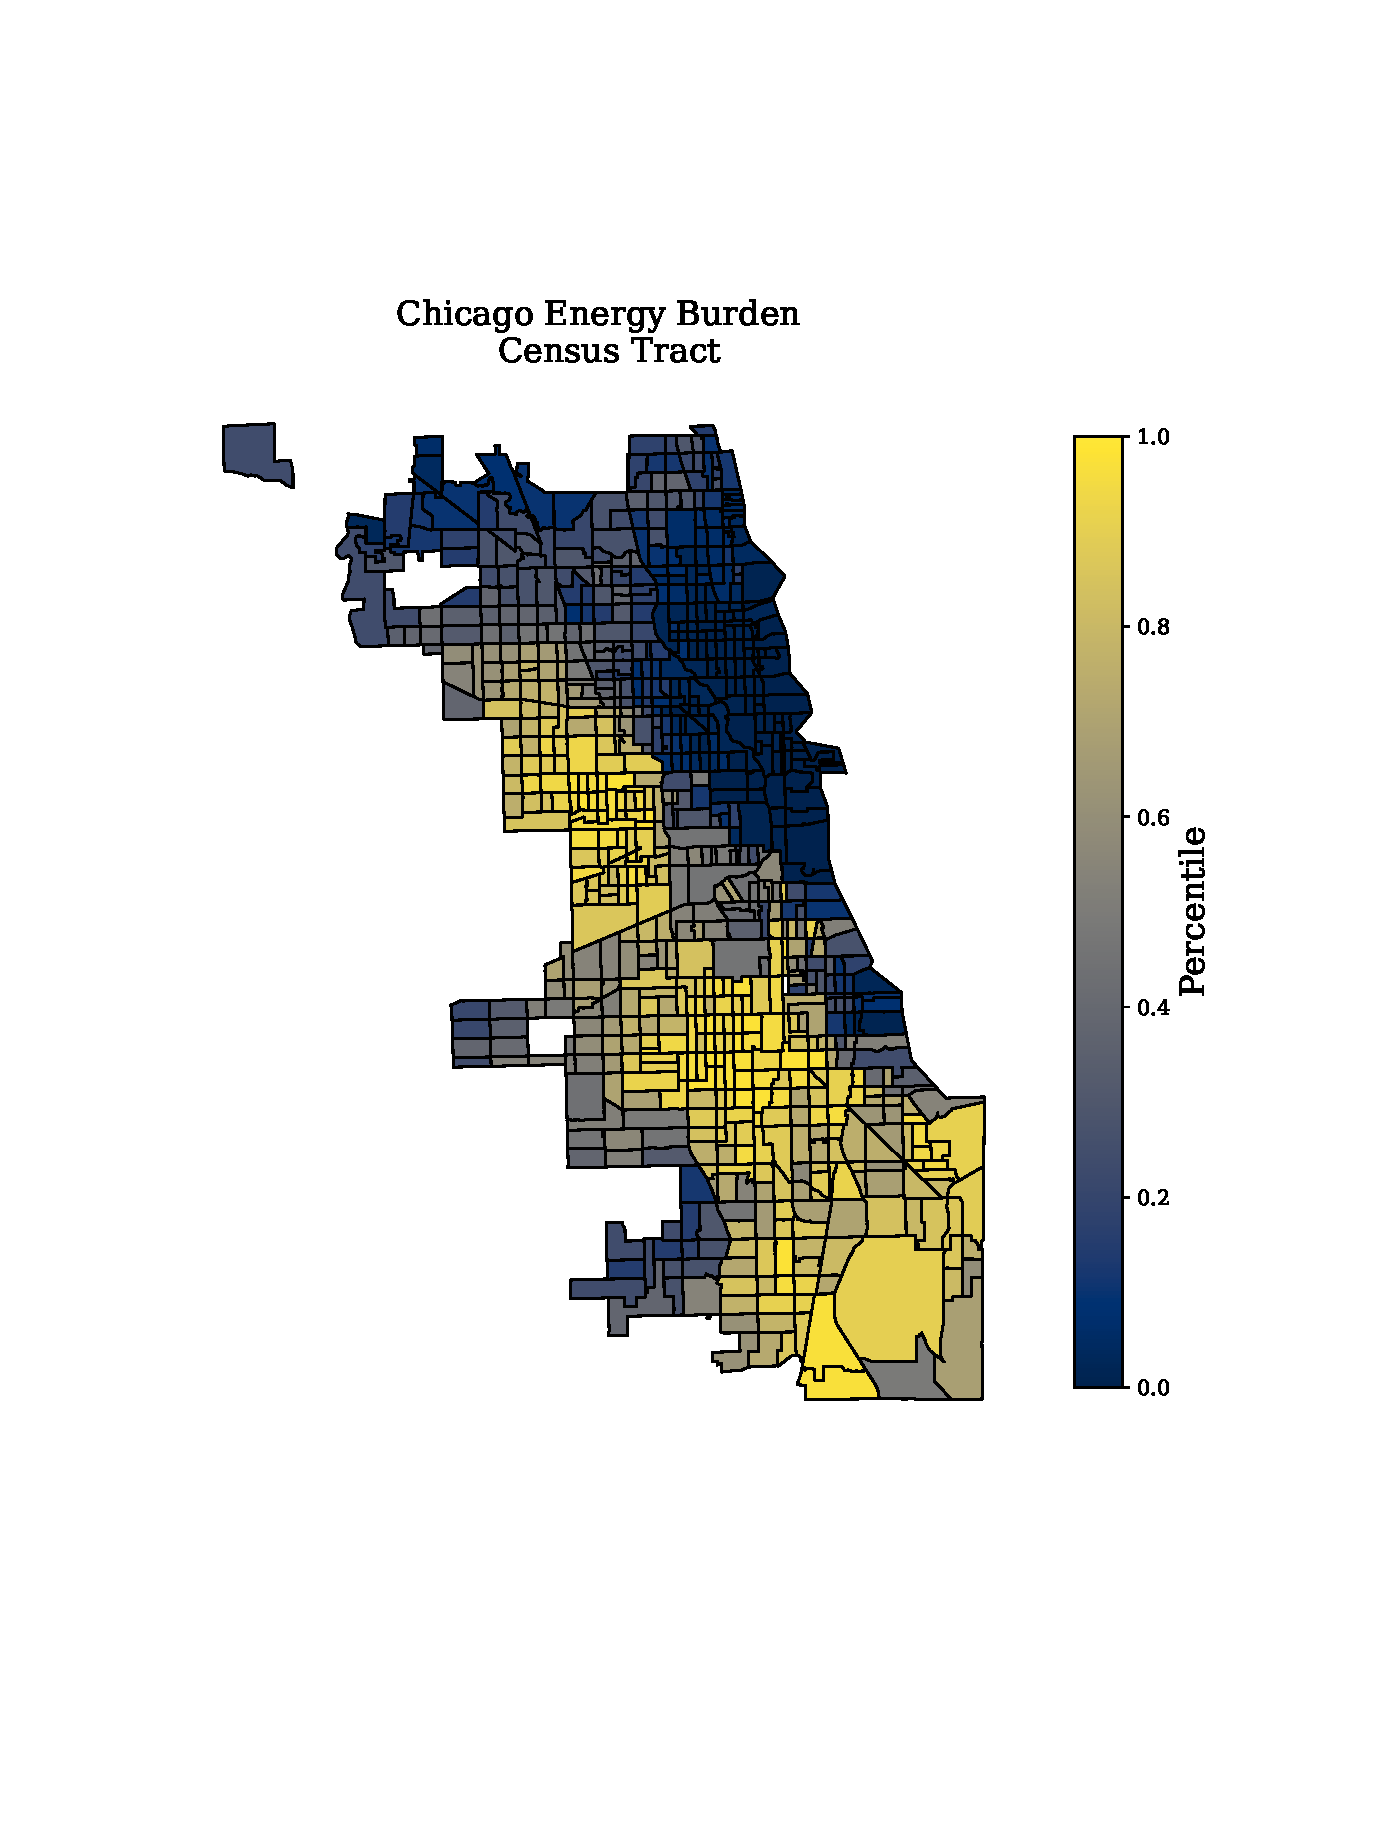
\includegraphics[width=\columnwidth]{energy_burden}
      \vspace*{-2cm}
      \caption{Energy burden throughout Chicago as a percentile. A region in the zeroth
      percentile has the least energy burden and a region in the 100th percentile has
      more energy burden than any other region.}
    \end{center}
\end{figure}

\subsubsection{Tree Canopy}

Urban tree cover effectively mitigate land surface temperatures in cities
\cite{loughner_roles_2012, schwaab_role_2021, mcdonald_tree_2021}. Tree canopy
reduces temperature by preventing ground heat storage through shade and encouraging
evapotranspiration \cite{mcdonald_tree_2021}. Thus, areas with greater tree cover
are less vulnerable heatwaves. Figure \ref{fig:tree_census} shows the distribution
of trees in Chicago from the Morton Arboretum Tree Census \cite{kua_chicago_2020}.

\begin{figure}[H]
  \label{fig:tree_census}
    \begin{center}
      \includegraphics[width=\columnwidth]{tree_canopy}
      \vspace*{-2cm}
      \caption{Distribution of trees in Chicago by percentile. A region in the zeroth
      percentile has the least tree canopy and a region in the 100th percentile has
      more tree cover than any other region.}
    \end{center}
\end{figure}


\section{Results}
\label{section:results}
After clustering the data with a hierarchical clustering algorithm, we developed
a map of the most similar regions according to their cluster. Figure \ref{fig:clustering}
shows these regions. The colors and numbers in Figure \ref{fig:clustering} simply
identify the cluster and do not correspond to heat wave risk nor priority.

\begin{figure}[H]
    \begin{center}
      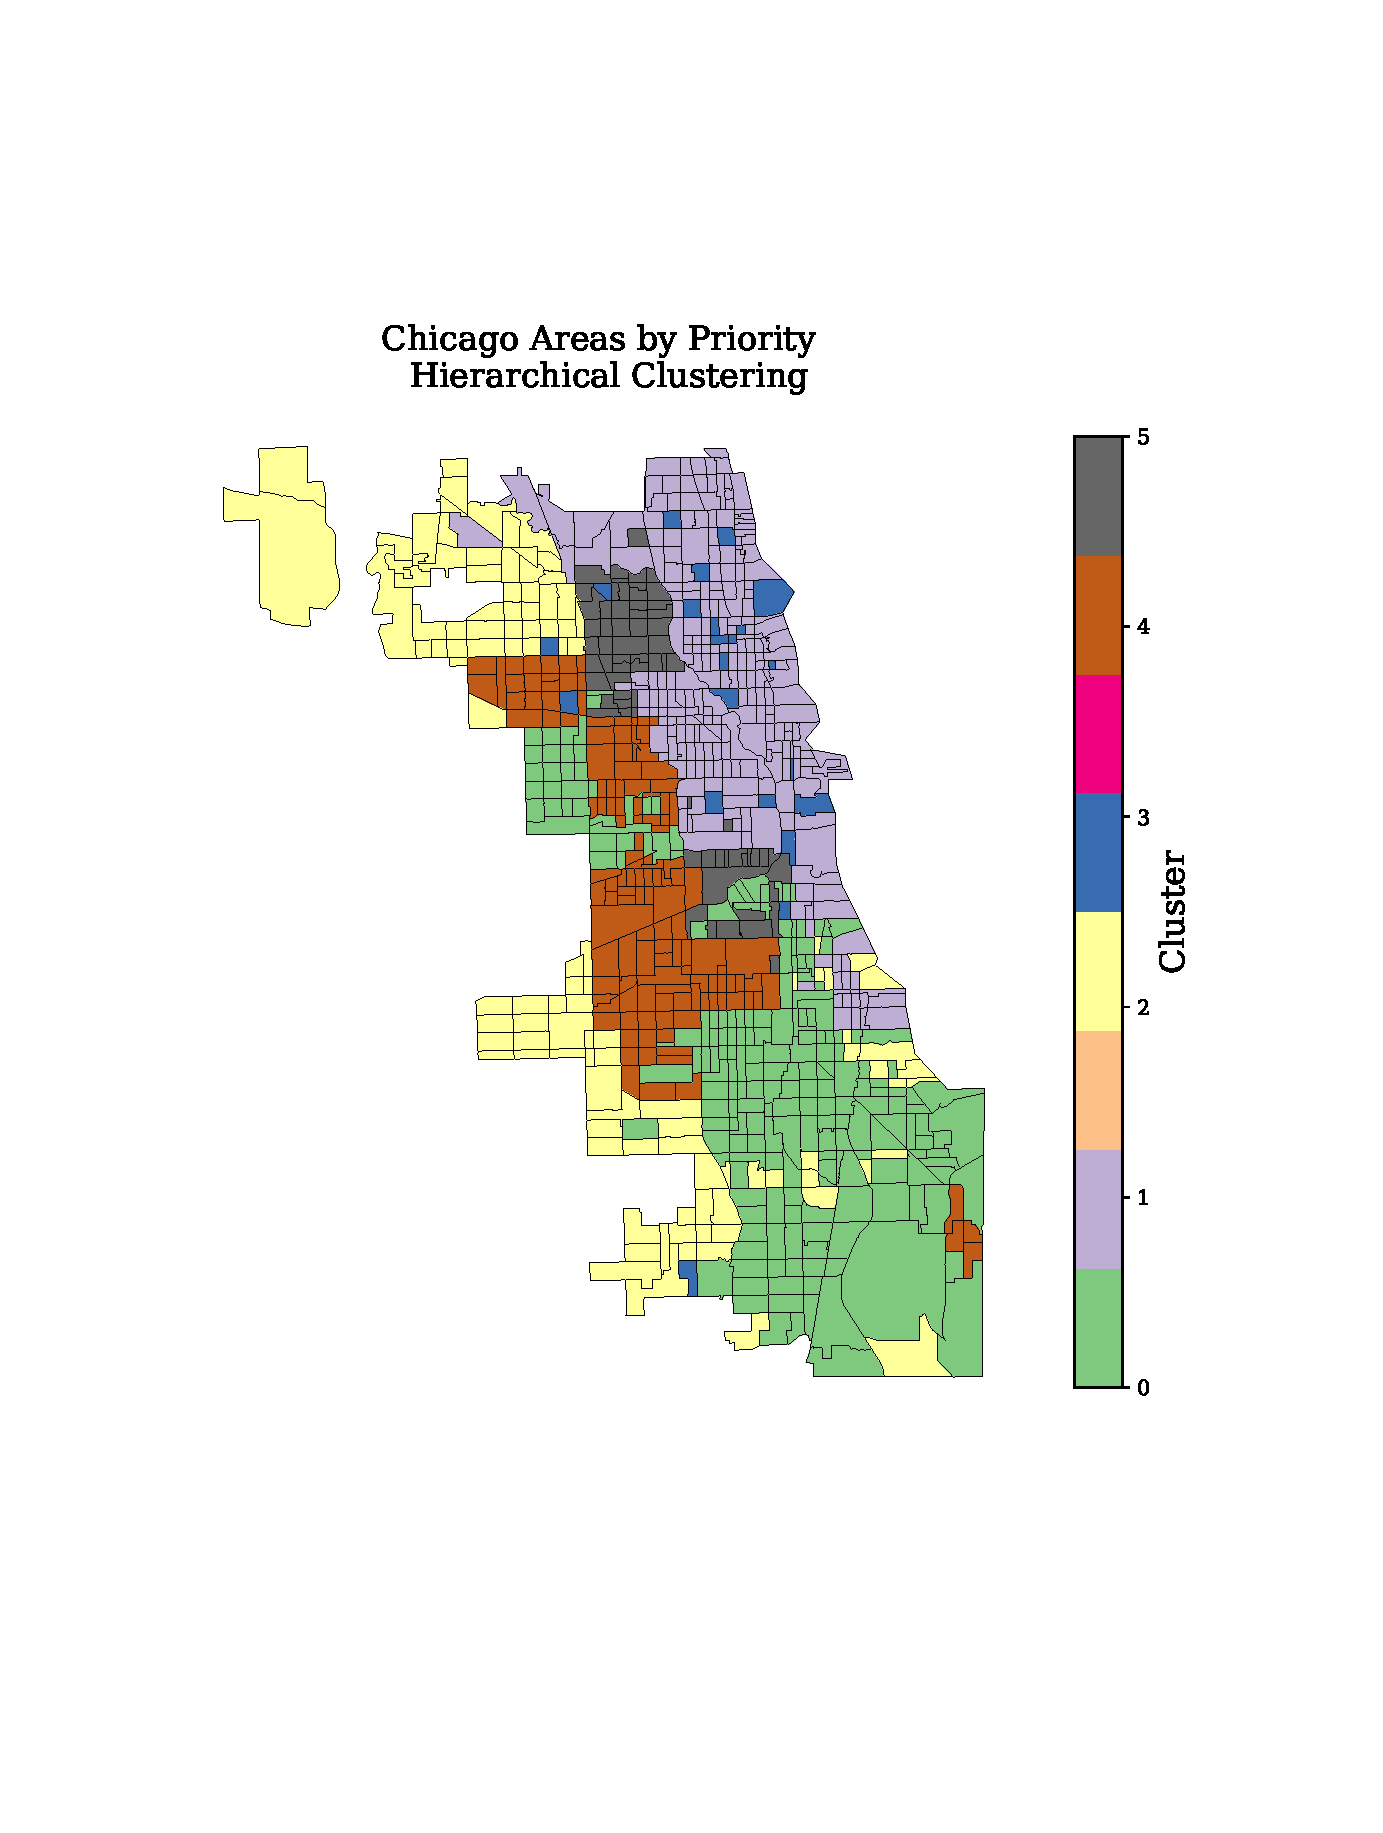
\includegraphics[trim=0 120 0 120, clip, width=\columnwidth]{clustering}
      % \vspace*{-3cm}
      \caption{The map of Chicago clusters. The numbers correspond to the order
      in which the algorithm created the groups and not the heatwave risk.}
      \label{fig:clustering}
    \end{center}
\end{figure}

Figure \ref{fig:cluster_compare} compares the mean vector of each cluster. The
colors and group numbers match the colors and group numbers from Figure
\ref{fig:clustering}.

\begin{figure}[H]
    \begin{center}
      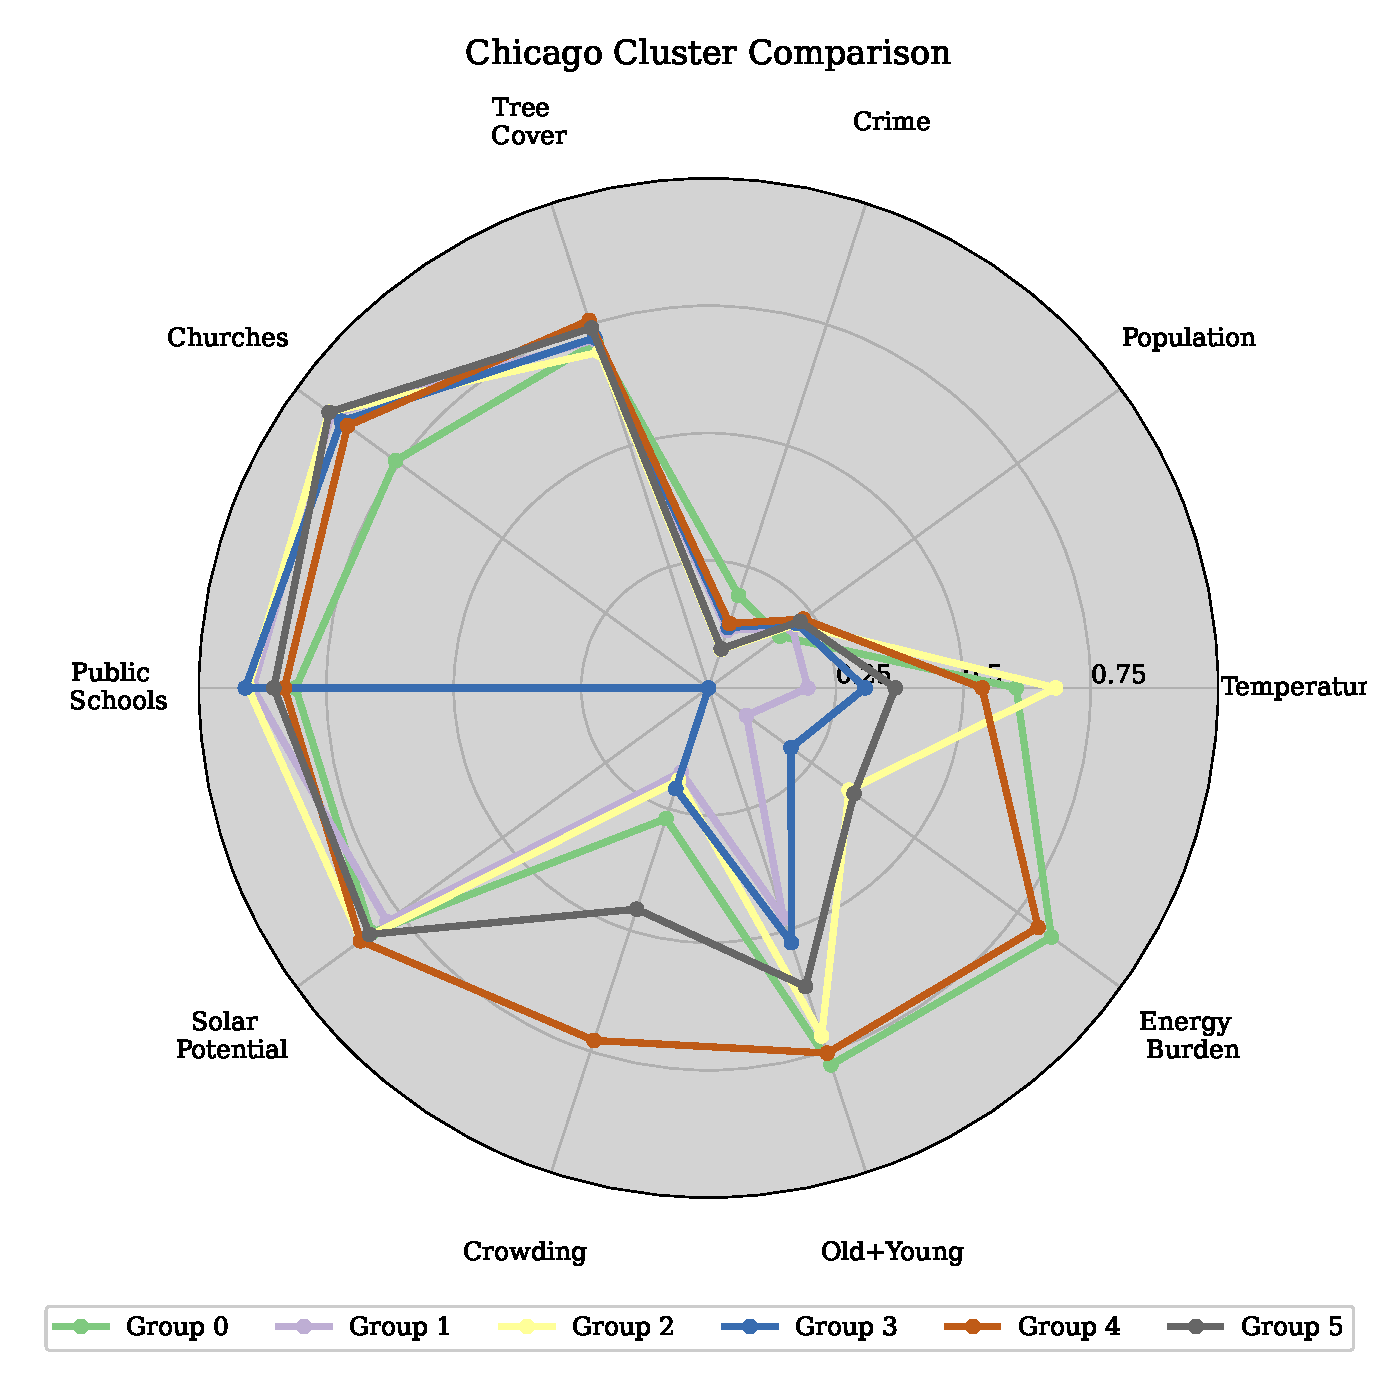
\includegraphics[width=0.95\columnwidth]{cluster_comparison}
      % \vspace*{-3cm}
      \caption{The map of Chicago clusters. The numbers correspond to the order
      in which the algorithm created the groups and not the heatwave risk.}
      \label{fig:cluster_compare}
    \end{center}
\end{figure}

There are several points of interest in Figure \ref{fig:cluster_compare}. First,
the average number of churches, public schools, crime rates, population, and tree
cover were similar across each cluster. The similarity in tree cover was unexpected
due to the strong effect of tree cover on temperature and \ac{uhi} noted in the
literature \cite{mcdonald_tree_2021,marando_urban_2022,schwaab_role_2021}. Further,
there was little difference in average crime rates across clusters. This is likely
due to the fact that a few census tracts had a much higher crime rate than all others.
With the exception of a single group, group 3, solar potential (i.e. the percent
of rooftops that qualify for solar panels \cite{google_project_2022}) was nearly
identical across all clusters.

Second, crowded housing, age, energy burden, and temperature were the most divergent
factors across the clusters. The key difference between the highest and second
highest priority clusters was crowding. It makes sense that the number of people
per household should be used to differentiate priority, \textit{ceteris paribus}.

The ``score'' that ranks the clusters is incidentally the area drawn by each
curve in Figure \ref{fig:cluster_compare}. The rank of each cluster is shown in
Figure \ref{fig:cluster_priority}.

\begin{figure}[H]
    \begin{center}
      \includegraphics[trim=0 200 0 120, clip, width=\columnwidth]{clustering_priority}
      % \vspace*{-3cm}
      \caption{The map of Chicago clusters according to priority.
      0 = Highest priority. 5 = Lowest priority.}
      \label{fig:cluster_priority}
    \end{center}
\end{figure}

The highest priority region (priority 0) are on the west side of the city, where
it is warmer, crowded, and energy burden is high. The areas closest to Lake Michigan
tend to be the coolest part of the city and the most affluent, thus making them
the lowest priority (priority 5) for rooftop solar panels.

\section{Discussion}
\label{section:discussion}
The prioritization mapping protocol outlined by this research is better suited for
identifying regions for targeted incentive distribution to address specific issues
in urban settings than existing general environmental justice community
identification tools currently used for funding dissemination.

\subsection{Comparison to other Energy Justice Mapping Tools}
Other screening tools have been developed to analyze spatial characteristics of
environmental justice. The \ac{ejscreen} tool from the \ac{epa} \cite{us_epa_ejscreen_2014}
and the US Council on Environmental Quality’s \ac{cejst} tool can both be used to
identify disadvantaged or vulnerable populations spatially
\cite{council_on_environmental_quality_climate_nodate}. However, the map generated
by this research identifies a more precise region of the city of Chicago to be
prioritized for rooftop solar initiatives, therefore informing more efficient
allocation of resources to the most vulnerable communities for this particular issue.
Figure \ref{fig:ejscreen_map} and Figure \ref{fig:cejst_map} show the at-risk areas
in Chicago identified by \ac{ejscreen} and \ac{cejst}, respectively.
\begin{figure}[H]
    \begin{center}
      \includegraphics[trim=0 200 0 120, clip, width=\columnwidth]{ejscreen_map}
      % \vspace*{-3cm}
      \caption{Environmental justice communities identified by \ac{ejscreen}. ``Yes''
      indicates that the community has environmental justice concerns.}
      \label{fig:ejscreen_map}
    \end{center}
\end{figure}

\begin{figure}[H]
    \begin{center}
      \includegraphics[trim=0 200 0 120, clip, width=\columnwidth]{cejst_map}
      % \vspace*{-3cm}
      \caption{Normalized energy burden from the \ac{cejst} tool.}
      \label{fig:cejst_map}
    \end{center}
\end{figure}

Importantly, neither of these tools incorporate heatwave risk and use a limited
set of social features. The prioritization created in this research considers
traditional environmental justice factors, including age, income, and race, but
also incorporates urban heat island impacts, qualified roof area, access to cooling
centers, tree cover, and energy burden to more specifically interrogate spatial
distribution of heat impacts that could be mitigated through access to cleaner,
cheaper energy for cooling. This is a more holistic approach to understanding
environmental justice for the specific issue of access to affordable energy to
cool urban homes in a heat wave. While mapping the distribution of spatial
attributes of environmental justice can illuminate inequities at a multitude of
scales, this more precise issue-specific mapping could be more effective for
policy and incentive development.

\subsection{Targeted Incentive Distribution}

Illinois \ac{sfa} is a state-funded program that “promotes equitable access to
the solar economy through program incentives that help make solar more affordable
for low-income communities” \cite{illinois_solar_for_all_environmental_2022}. The
program allows low-income communities to benefit from community solar arrays and
distributed generation installations, as well as providing low-cost solar
installations to non-profit organizations and public facilities. Initial funding
for SFA was provided by Illinois' 2017 Future Energy Jobs Act, but when funds were
exhausted, talk of a “solar cliff” highlighted the uncertainty of the future of
solar incentives in the state (Lydersen, 2020). The popularity of this program
and limited funding for solar projects emphasizes the need for targeted distribution
of funds to the communities that need it most.

SFA has an explicit commitment to increasing access to solar energy among
environmental justice communities. SFA uses \ac{epa}’s \ac{ejscreen} and a
self-designation  process to identify environmental justice communities across
the state of Illinois. However, this method of identifying communities to target
for SFA incentives is based on a more general understanding of environmental
justice, and does not necessarily consider the potential impact of solar energy
to reduce the energy burden on low-income households through solar installation.
Targeted prioritization as outlined in this research could result in allocation
of limited solar incentive funds to the communities that would experience the
greatest benefit from solar installations by reducing risks associated with heatwaves.

\subsection{Limitations}

This study curated census and satellite data to develop a heat wave risk prioritization
scheme. There are some limitations to this process. First, we implicitly weight
vulnerability factors higher than hazard or exposure since we have more of those
data points. Second, the heat wave temperature anomaly does not account for duration
in the definition of heat wave. We also only consider temperature as a heat wave
hazard. Other climatic factors may influence the effect of heat waves and heat
stress on the human body, such as humidity. These issues may be addressed by
adding more data points and improving the resolution of the data. Finally, stronger
models relating proximal mechanisms, such as crime rate and isolation, to negative
heat wave outcomes would be useful in weighting each variable.


\section{Conclusion}
Limitations:
\begin{enumerate}
  \item we implicitly weight vulnerability factors higher than hazard or exposure since we have more of those data points.
  \item the heatwave temperature anomaly does not factor in duration in the definition
  of heatwave.
  \item we only consider temperature as a heatwave hazard. Other climatic factors
  may influence the effect of heatwaves and heat stress on the human body. Such as
  humidity.
\end{enumerate}

The argument advanced in this work is that prioritizing the distribution of solar
panels offered by programs like Solar for All or Illinois Shines will minimize the
overall heat-related adversity. Current standards for prioritizing beneficiaries
of these programs do not account for climate hazards such as heatwaves nor the
many vulnerabilities that, together, create a holistic understanding of risk.


% \bibliography
\section*{References}
\bibliographystyle{myunsrt}
\bibliography{bibliography_software}

 \end{document}
